% Generated from the unchanged rq3-cells.csv. All 27 contracts appear.
\begin{figure}[!htbp]
\centering
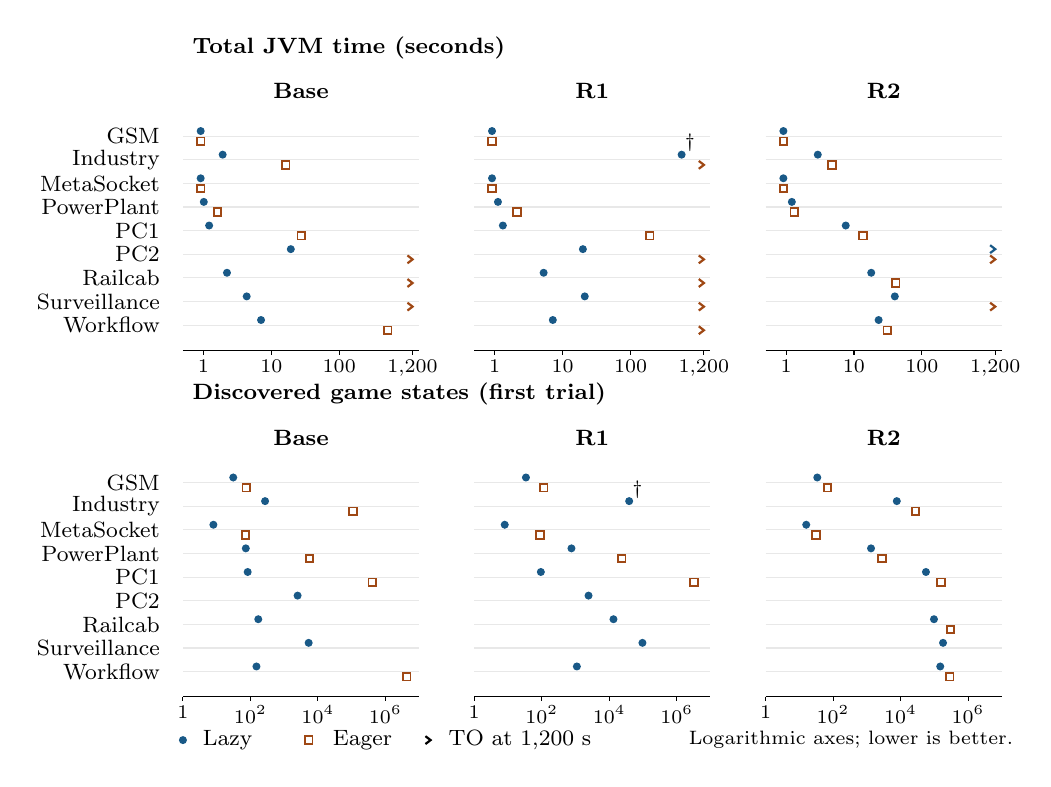
\begin{tikzpicture}[x=1cm,y=1cm,font=\footnotesize]
\definecolor{lazy}{RGB}{25,89,135}
\definecolor{eager}{RGB}{159,72,20}
\node[anchor=west,font=\footnotesize\bfseries] at (2,1.12) {Total JVM time (seconds)};
\node[font=\footnotesize\bfseries] at (3.5,0.57) {Base};
\node[anchor=east] at (1.83,0.0) {GSM};
\draw[black!9] (2.0,0.0)--(5.0,0.0);
% gsm/base/lazy: JVM median/min/max = 0.9130392/0.9125639/0.9132812
\draw[lazy,line width=.7pt] (2.22544,0.06500)--(2.22573,0.06500);
\fill[lazy] (2.22563,0.06500) circle (1.45pt);
% gsm/base/eager: JVM median/min/max = 0.9131794/0.9126908/0.9143673
\draw[eager,line width=.7pt] (2.22549,-0.06500)--(2.22618,-0.06500);
\draw[eager,fill=white,line width=.65pt] (2.17769,-0.11300) rectangle (2.27369,-0.01700);
\node[anchor=east] at (1.83,-0.3) {Industry};
\draw[black!9] (2.0,-0.3)--(5.0,-0.3);
% industry/base/lazy: JVM median/min/max = 1.9232429/1.9213733/1.9245728
\draw[lazy,line width=.7pt] (2.50442,-0.23500)--(2.50504,-0.23500);
\fill[lazy] (2.50478,-0.23500) circle (1.45pt);
% industry/base/eager: JVM median/min/max = 16.3326169/16.0183602/16.5217978
\draw[eager,line width=.7pt] (3.29905,-0.36500)--(3.31064,-0.36500);
\draw[eager,fill=white,line width=.65pt] (3.25833,-0.41300) rectangle (3.35433,-0.31700);
\node[anchor=east] at (1.83,-0.6) {MetaSocket};
\draw[black!9] (2.0,-0.6)--(5.0,-0.6);
% metasocket/base/lazy: JVM median/min/max = 0.9123447/0.8130894/0.9141439
\draw[lazy,line width=.7pt] (2.18219,-0.53500)--(2.22609,-0.53500);
\fill[lazy] (2.22535,-0.53500) circle (1.45pt);
% metasocket/base/eager: JVM median/min/max = 0.9137026/0.9102252/0.9147436
\draw[eager,line width=.7pt] (2.22448,-0.66500)--(2.22633,-0.66500);
\draw[eager,fill=white,line width=.65pt] (2.17791,-0.71300) rectangle (2.27391,-0.61700);
\node[anchor=east] at (1.83,-0.8999999999999999) {PowerPlant};
\draw[black!9] (2.0,-0.8999999999999999)--(5.0,-0.8999999999999999);
% powerplant/base/lazy: JVM median/min/max = 1.0144494/1.0141636/1.0154832
\draw[lazy,line width=.7pt] (2.26499,-0.83500)--(2.26548,-0.83500);
\fill[lazy] (2.26510,-0.83500) circle (1.45pt);
% powerplant/base/eager: JVM median/min/max = 1.618809/1.5183377/1.6203611
\draw[eager,line width=.7pt] (2.41620,-0.96500)--(2.44057,-0.96500);
\draw[eager,fill=white,line width=.65pt] (2.39221,-1.01300) rectangle (2.48821,-0.91700);
\node[anchor=east] at (1.83,-1.2) {PC1};
\draw[black!9] (2.0,-1.2)--(5.0,-1.2);
% productioncell_arms1/base/lazy: JVM median/min/max = 1.2159295/1.2146609/1.2171044
\draw[lazy,line width=.7pt] (2.33259,-1.13500)--(2.33334,-1.13500);
\fill[lazy] (2.33298,-1.13500) circle (1.45pt);
% productioncell_arms1/base/eager: JVM median/min/max = 27.6003525/27.2324243/28.5102851
\draw[eager,line width=.7pt] (3.49789,-1.26500)--(3.51507,-1.26500);
\draw[eager,fill=white,line width=.65pt] (3.45492,-1.31300) rectangle (3.55092,-1.21700);
\node[anchor=east] at (1.83,-1.5) {PC2};
\draw[black!9] (2.0,-1.5)--(5.0,-1.5);
% productioncell_arms2/base/lazy: JVM median/min/max = 19.3573477/19.1537231/19.8590448
\draw[lazy,line width=.7pt] (3.36603,-1.43500)--(3.37958,-1.43500);
\fill[lazy] (3.36999,-1.43500) circle (1.45pt);
\draw[eager,line width=.8pt] (4.85139,-1.61500)--(4.91639,-1.56500)--(4.85139,-1.51500);
\node[anchor=east] at (1.83,-1.7999999999999998) {Railcab};
\draw[black!9] (2.0,-1.7999999999999998)--(5.0,-1.7999999999999998);
% railcab/base/lazy: JVM median/min/max = 2.2257407/2.2238686/2.2280735
\draw[lazy,line width=.7pt] (2.55920,-1.73500)--(2.55991,-1.73500);
\fill[lazy] (2.55952,-1.73500) circle (1.45pt);
\draw[eager,line width=.8pt] (4.85139,-1.91500)--(4.91639,-1.86500)--(4.85139,-1.81500);
\node[anchor=east] at (1.83,-2.1) {Surveillance};
\draw[black!9] (2.0,-2.1)--(5.0,-2.1);
% surveillance/base/lazy: JVM median/min/max = 4.3426951/4.3404821/4.442846
\draw[lazy,line width=.7pt] (2.80978,-2.03500)--(2.81851,-2.03500);
\fill[lazy] (2.80997,-2.03500) circle (1.45pt);
\draw[eager,line width=.8pt] (4.85139,-2.21500)--(4.91639,-2.16500)--(4.85139,-2.11500);
\node[anchor=east] at (1.83,-2.4) {Workflow};
\draw[black!9] (2.0,-2.4)--(5.0,-2.4);
% workflow/base/lazy: JVM median/min/max = 7.0619707/6.9637387/7.0643322
\draw[lazy,line width=.7pt] (2.98691,-2.33500)--(2.99229,-2.33500);
\fill[lazy] (2.99216,-2.33500) circle (1.45pt);
% workflow/base/eager: JVM median/min/max = 518.0498148/501.4345891/528.424175
\draw[eager,line width=.7pt] (4.58942,-2.46500)--(4.60907,-2.46500);
\draw[eager,fill=white,line width=.65pt] (4.55364,-2.51300) rectangle (4.64964,-2.41700);
\draw (2.0,-2.72)--(5.0,-2.72);
\draw (2.25972,-2.72)--(2.25972,-2.7750000000000004);
\node[anchor=north,font=\scriptsize,inner sep=1pt] at (2.25972,-2.7950000000000004) {1};
\draw (3.12251,-2.72)--(3.12251,-2.7750000000000004);
\node[anchor=north,font=\scriptsize,inner sep=1pt] at (3.12251,-2.7950000000000004) {10};
\draw (3.98529,-2.72)--(3.98529,-2.7750000000000004);
\node[anchor=north,font=\scriptsize,inner sep=1pt] at (3.98529,-2.7950000000000004) {100};
\draw (4.91639,-2.72)--(4.91639,-2.7750000000000004);
\node[anchor=north,font=\scriptsize,inner sep=1pt] at (4.91639,-2.7950000000000004) {1,200};
\node[font=\footnotesize\bfseries] at (7.2,0.57) {R1};
\draw[black!9] (5.7,0.0)--(8.7,0.0);
% gsm/r1/lazy: JVM median/min/max = 0.9130627/0.9123974/0.9144691
\draw[lazy,line width=.7pt] (5.92537,0.06500)--(5.92622,0.06500);
\fill[lazy] (5.92564,0.06500) circle (1.45pt);
% gsm/r1/eager: JVM median/min/max = 0.9133292/0.9125619/0.9142938
\draw[eager,line width=.7pt] (5.92544,-0.06500)--(5.92615,-0.06500);
\draw[eager,fill=white,line width=.65pt] (5.87775,-0.11300) rectangle (5.97375,-0.01700);
\draw[black!9] (5.7,-0.3)--(8.7,-0.3);
% industry/r1/lazy: JVM median/min/max = 563.926891/536.104858/568.0240798
\draw[lazy,line width=.7pt] (8.31447,-0.23500)--(8.33614,-0.23500);
\fill[lazy] (8.33343,-0.23500) circle (1.45pt);
\node[font=\scriptsize,anchor=south west,inner sep=1pt] at (8.33343,-0.23500) {$\dagger$};
\draw[eager,line width=.8pt] (8.55139,-0.41500)--(8.61639,-0.36500)--(8.55139,-0.31500);
\draw[black!9] (5.7,-0.6)--(8.7,-0.6);
% metasocket/r1/lazy: JVM median/min/max = 0.9127905/0.9125641/0.9131296
\draw[lazy,line width=.7pt] (5.92544,-0.53500)--(5.92567,-0.53500);
\fill[lazy] (5.92553,-0.53500) circle (1.45pt);
% metasocket/r1/eager: JVM median/min/max = 0.9139618/0.9136255/0.914775
\draw[eager,line width=.7pt] (5.92587,-0.66500)--(5.92635,-0.66500);
\draw[eager,fill=white,line width=.65pt] (5.87801,-0.71300) rectangle (5.97401,-0.61700);
\draw[black!9] (5.7,-0.8999999999999999)--(8.7,-0.8999999999999999);
% powerplant/r1/lazy: JVM median/min/max = 1.1158616/1.1153371/1.1176993
\draw[lazy,line width=.7pt] (6.00062,-0.83500)--(6.00142,-0.83500);
\fill[lazy] (6.00080,-0.83500) circle (1.45pt);
% powerplant/r1/eager: JVM median/min/max = 2.1260115/2.0235737/2.1266509
\draw[eager,line width=.7pt] (6.22384,-0.96500)--(6.24245,-0.96500);
\draw[eager,fill=white,line width=.65pt] (6.19434,-1.01300) rectangle (6.29034,-0.91700);
\draw[black!9] (5.7,-1.2)--(8.7,-1.2);
% productioncell_arms1/r1/lazy: JVM median/min/max = 1.3185895/1.31351/1.3191768
\draw[lazy,line width=.7pt] (6.06191,-1.13500)--(6.06352,-1.13500);
\fill[lazy] (6.06335,-1.13500) circle (1.45pt);
% productioncell_arms1/r1/eager: JVM median/min/max = 190.9923827/187.8600834/192.6318621
\draw[eager,line width=.7pt] (7.92155,-1.26500)--(7.93095,-1.26500);
\draw[eager,fill=white,line width=.65pt] (7.87974,-1.31300) rectangle (7.97574,-1.21700);
\draw[black!9] (5.7,-1.5)--(8.7,-1.5);
% productioncell_arms2/r1/lazy: JVM median/min/max = 19.856803/19.6565302/20.2649448
\draw[lazy,line width=.7pt] (7.07574,-1.43500)--(7.08716,-1.43500);
\fill[lazy] (7.07954,-1.43500) circle (1.45pt);
\draw[eager,line width=.8pt] (8.55139,-1.61500)--(8.61639,-1.56500)--(8.55139,-1.51500);
\draw[black!9] (5.7,-1.7999999999999998)--(8.7,-1.7999999999999998);
% railcab/r1/lazy: JVM median/min/max = 5.2488108/5.24175/5.2504391
\draw[lazy,line width=.7pt] (6.58048,-1.73500)--(6.58110,-1.73500);
\fill[lazy] (6.58098,-1.73500) circle (1.45pt);
\draw[eager,line width=.8pt] (8.55139,-1.91500)--(8.61639,-1.86500)--(8.55139,-1.81500);
\draw[black!9] (5.7,-2.1)--(8.7,-2.1);
% surveillance/r1/lazy: JVM median/min/max = 21.157874/20.768775/21.266785
\draw[lazy,line width=.7pt] (7.09636,-2.03500)--(7.10524,-2.03500);
\fill[lazy] (7.10332,-2.03500) circle (1.45pt);
\draw[eager,line width=.8pt] (8.55139,-2.21500)--(8.61639,-2.16500)--(8.55139,-2.11500);
\draw[black!9] (5.7,-2.4)--(8.7,-2.4);
% workflow/r1/lazy: JVM median/min/max = 7.1662477/7.0585443/7.2598173
\draw[lazy,line width=.7pt] (6.69198,-2.33500)--(6.70252,-2.33500);
\fill[lazy] (6.69765,-2.33500) circle (1.45pt);
\draw[eager,line width=.8pt] (8.55139,-2.51500)--(8.61639,-2.46500)--(8.55139,-2.41500);
\draw (5.7,-2.72)--(8.7,-2.72);
\draw (5.95972,-2.72)--(5.95972,-2.7750000000000004);
\node[anchor=north,font=\scriptsize,inner sep=1pt] at (5.95972,-2.7950000000000004) {1};
\draw (6.82251,-2.72)--(6.82251,-2.7750000000000004);
\node[anchor=north,font=\scriptsize,inner sep=1pt] at (6.82251,-2.7950000000000004) {10};
\draw (7.68529,-2.72)--(7.68529,-2.7750000000000004);
\node[anchor=north,font=\scriptsize,inner sep=1pt] at (7.68529,-2.7950000000000004) {100};
\draw (8.61639,-2.72)--(8.61639,-2.7750000000000004);
\node[anchor=north,font=\scriptsize,inner sep=1pt] at (8.61639,-2.7950000000000004) {1,200};
\node[font=\footnotesize\bfseries] at (10.9,0.57) {R2};
\draw[black!9] (9.4,0.0)--(12.4,0.0);
% gsm/r2/lazy: JVM median/min/max = 0.9135891/0.9123249/0.9146305
\draw[lazy,line width=.7pt] (9.62534,0.06500)--(9.62629,0.06500);
\fill[lazy] (9.62586,0.06500) circle (1.45pt);
% gsm/r2/eager: JVM median/min/max = 0.9138196/0.9137006/0.9140096
\draw[eager,line width=.7pt] (9.62591,-0.06500)--(9.62603,-0.06500);
\draw[eager,fill=white,line width=.65pt] (9.57795,-0.11300) rectangle (9.67395,-0.01700);
\draw[black!9] (9.4,-0.3)--(12.4,-0.3);
% industry/r2/lazy: JVM median/min/max = 2.9308907/2.9296067/2.9327077
\draw[lazy,line width=.7pt] (10.06248,-0.23500)--(10.06287,-0.23500);
\fill[lazy] (10.06264,-0.23500) circle (1.45pt);
% industry/r2/eager: JVM median/min/max = 4.7461032/4.7437719/4.9516504
\draw[eager,line width=.7pt] (10.24307,-0.36500)--(10.25914,-0.36500);
\draw[eager,fill=white,line width=.65pt] (10.19526,-0.41300) rectangle (10.29126,-0.31700);
\draw[black!9] (9.4,-0.6)--(12.4,-0.6);
% metasocket/r2/lazy: JVM median/min/max = 0.9132551/0.9130302/0.9140156
\draw[lazy,line width=.7pt] (9.62563,-0.53500)--(9.62603,-0.53500);
\fill[lazy] (9.62572,-0.53500) circle (1.45pt);
% metasocket/r2/eager: JVM median/min/max = 0.913473/0.9128511/0.9139487
\draw[eager,line width=.7pt] (9.62556,-0.66500)--(9.62601,-0.66500);
\draw[eager,fill=white,line width=.65pt] (9.57781,-0.71300) rectangle (9.67381,-0.61700);
\draw[black!9] (9.4,-0.8999999999999999)--(12.4,-0.8999999999999999);
% powerplant/r2/lazy: JVM median/min/max = 1.2168166/1.215708/1.2173083
\draw[lazy,line width=.7pt] (9.73291,-0.83500)--(9.73341,-0.83500);
\fill[lazy] (9.73325,-0.83500) circle (1.45pt);
% powerplant/r2/eager: JVM median/min/max = 1.3178143/1.3166207/1.3182642
\draw[eager,line width=.7pt] (9.76279,-0.96500)--(9.76326,-0.96500);
\draw[eager,fill=white,line width=.65pt] (9.71513,-1.01300) rectangle (9.81113,-0.91700);
\draw[black!9] (9.4,-1.2)--(12.4,-1.2);
% productioncell_arms1/r2/lazy: JVM median/min/max = 7.5612511/7.4619858/8.2725932
\draw[lazy,line width=.7pt] (10.41281,-1.13500)--(10.45145,-1.13500);
\fill[lazy] (10.41776,-1.13500) circle (1.45pt);
% productioncell_arms1/r2/eager: JVM median/min/max = 13.611786/13.5977826/14.1108414
\draw[eager,line width=.7pt] (10.63766,-1.26500)--(10.65154,-1.26500);
\draw[eager,fill=white,line width=.65pt] (10.59005,-1.31300) rectangle (10.68605,-1.21700);
\draw[black!9] (9.4,-1.5)--(12.4,-1.5);
\draw[lazy,line width=.8pt] (12.25139,-1.48500)--(12.31639,-1.43500)--(12.25139,-1.38500);
\draw[eager,line width=.8pt] (12.25139,-1.61500)--(12.31639,-1.56500)--(12.25139,-1.51500);
\draw[black!9] (9.4,-1.7999999999999998)--(12.4,-1.7999999999999998);
% railcab/r2/lazy: JVM median/min/max = 17.933768/17.8337679/17.9398622
\draw[lazy,line width=.7pt] (10.73927,-1.73500)--(10.74150,-1.73500);
\fill[lazy] (10.74137,-1.73500) circle (1.45pt);
% railcab/r2/eager: JVM median/min/max = 41.1987655/41.1810933/41.3951525
\draw[eager,line width=.7pt] (11.05286,-1.86500)--(11.05480,-1.86500);
\draw[eager,fill=white,line width=.65pt] (11.00502,-1.91300) rectangle (11.10102,-1.81700);
\draw[black!9] (9.4,-2.1)--(12.4,-2.1);
% surveillance/r2/lazy: JVM median/min/max = 39.8928114/39.8765955/40.3825681
\draw[lazy,line width=.7pt] (11.04080,-2.03500)--(11.04552,-2.03500);
\fill[lazy] (11.04095,-2.03500) circle (1.45pt);
\draw[eager,line width=.8pt] (12.25139,-2.21500)--(12.31639,-2.16500)--(12.25139,-2.11500);
\draw[black!9] (9.4,-2.4)--(12.4,-2.4);
% workflow/r2/lazy: JVM median/min/max = 23.0530876/22.7744215/23.3715254
\draw[lazy,line width=.7pt] (10.83091,-2.33500)--(10.84060,-2.33500);
\fill[lazy] (10.83546,-2.33500) circle (1.45pt);
% workflow/r2/eager: JVM median/min/max = 30.9360675/30.4163997/31.6364434
\draw[eager,line width=.7pt] (10.93932,-2.46500)--(10.95406,-2.46500);
\draw[eager,fill=white,line width=.65pt] (10.89767,-2.51300) rectangle (10.99367,-2.41700);
\draw (9.4,-2.72)--(12.4,-2.72);
\draw (9.65972,-2.72)--(9.65972,-2.7750000000000004);
\node[anchor=north,font=\scriptsize,inner sep=1pt] at (9.65972,-2.7950000000000004) {1};
\draw (10.52251,-2.72)--(10.52251,-2.7750000000000004);
\node[anchor=north,font=\scriptsize,inner sep=1pt] at (10.52251,-2.7950000000000004) {10};
\draw (11.38529,-2.72)--(11.38529,-2.7750000000000004);
\node[anchor=north,font=\scriptsize,inner sep=1pt] at (11.38529,-2.7950000000000004) {100};
\draw (12.31639,-2.72)--(12.31639,-2.7750000000000004);
\node[anchor=north,font=\scriptsize,inner sep=1pt] at (12.31639,-2.7950000000000004) {1,200};
\node[anchor=west,font=\footnotesize\bfseries] at (2,-3.2800000000000002) {Discovered game states (first trial)};
\node[font=\footnotesize\bfseries] at (3.5,-3.8300000000000005) {Base};
\node[anchor=east] at (1.83,-4.4) {GSM};
\draw[black!9] (2.0,-4.4)--(5.0,-4.4);
% gsm/base/lazy: first-trial states = 31
\fill[lazy] (2.63916,-4.33500) circle (1.45pt);
% gsm/base/eager: first-trial states = 75
\draw[eager,fill=white,line width=.65pt] (2.75560,-4.51300) rectangle (2.85160,-4.41700);
\node[anchor=east] at (1.83,-4.7) {Industry};
\draw[black!9] (2.0,-4.7)--(5.0,-4.7);
% industry/base/lazy: first-trial states = 272
\fill[lazy] (3.04339,-4.63500) circle (1.45pt);
% industry/base/eager: first-trial states = 109726
\draw[eager,fill=white,line width=.65pt] (4.11213,-4.81300) rectangle (4.20813,-4.71700);
\node[anchor=east] at (1.83,-5.0) {MetaSocket};
\draw[black!9] (2.0,-5.0)--(5.0,-5.0);
% metasocket/base/lazy: first-trial states = 8
\fill[lazy] (2.38704,-4.93500) circle (1.45pt);
% metasocket/base/eager: first-trial states = 71
\draw[eager,fill=white,line width=.65pt] (2.74540,-5.11300) rectangle (2.84140,-5.01700);
\node[anchor=east] at (1.83,-5.300000000000001) {PowerPlant};
\draw[black!9] (2.0,-5.300000000000001)--(5.0,-5.300000000000001);
% powerplant/base/lazy: first-trial states = 73
\fill[lazy] (2.79857,-5.23500) circle (1.45pt);
% powerplant/base/eager: first-trial states = 5634
\draw[eager,fill=white,line width=.65pt] (3.55949,-5.41300) rectangle (3.65549,-5.31700);
\node[anchor=east] at (1.83,-5.6000000000000005) {PC1};
\draw[black!9] (2.0,-5.6000000000000005)--(5.0,-5.6000000000000005);
% productioncell_arms1/base/lazy: first-trial states = 83
\fill[lazy] (2.82246,-5.53500) circle (1.45pt);
% productioncell_arms1/base/eager: first-trial states = 407019
\draw[eager,fill=white,line width=.65pt] (4.35612,-5.71300) rectangle (4.45212,-5.61700);
\node[anchor=east] at (1.83,-5.9) {PC2};
\draw[black!9] (2.0,-5.9)--(5.0,-5.9);
% productioncell_arms2/base/lazy: first-trial states = 2502
\fill[lazy] (3.45641,-5.83500) circle (1.45pt);
\node[anchor=east] at (1.83,-6.2) {Railcab};
\draw[black!9] (2.0,-6.2)--(5.0,-6.2);
% railcab/base/lazy: first-trial states = 171
\fill[lazy] (2.95700,-6.13500) circle (1.45pt);
\node[anchor=east] at (1.83,-6.5) {Surveillance};
\draw[black!9] (2.0,-6.5)--(5.0,-6.5);
% surveillance/base/lazy: first-trial states = 5319
\fill[lazy] (3.59678,-6.43500) circle (1.45pt);
\node[anchor=east] at (1.83,-6.800000000000001) {Workflow};
\draw[black!9] (2.0,-6.800000000000001)--(5.0,-6.800000000000001);
% workflow/base/lazy: first-trial states = 151
\fill[lazy] (2.93385,-6.73500) circle (1.45pt);
% workflow/base/eager: first-trial states = 4292588
\draw[eager,fill=white,line width=.65pt] (4.79459,-6.91300) rectangle (4.89059,-6.81700);
\draw (2.0,-7.120000000000001)--(5.0,-7.120000000000001);
\draw (2.00000,-7.120000000000001)--(2.00000,-7.175000000000001);
\node[anchor=north,font=\scriptsize,inner sep=1pt] at (2.00000,-7.195000000000001) {1};
\draw (2.85714,-7.120000000000001)--(2.85714,-7.175000000000001);
\node[anchor=north,font=\scriptsize,inner sep=1pt] at (2.85714,-7.195000000000001) {$10^2$};
\draw (3.71429,-7.120000000000001)--(3.71429,-7.175000000000001);
\node[anchor=north,font=\scriptsize,inner sep=1pt] at (3.71429,-7.195000000000001) {$10^4$};
\draw (4.57143,-7.120000000000001)--(4.57143,-7.175000000000001);
\node[anchor=north,font=\scriptsize,inner sep=1pt] at (4.57143,-7.195000000000001) {$10^6$};
\node[font=\footnotesize\bfseries] at (7.2,-3.8300000000000005) {R1};
\draw[black!9] (5.7,-4.4)--(8.7,-4.4);
% gsm/r1/lazy: first-trial states = 34
\fill[lazy] (6.35635,-4.33500) circle (1.45pt);
% gsm/r1/eager: first-trial states = 114
\draw[eager,fill=white,line width=.65pt] (6.53353,-4.51300) rectangle (6.62953,-4.41700);
\draw[black!9] (5.7,-4.7)--(8.7,-4.7);
% industry/r1/lazy: first-trial states = 38942
\fill[lazy] (7.66732,-4.63500) circle (1.45pt);
\node[font=\scriptsize,anchor=south west,inner sep=1pt] at (7.66732,-4.63500) {$\dagger$};
\draw[black!9] (5.7,-5.0)--(8.7,-5.0);
% metasocket/r1/lazy: first-trial states = 8
\fill[lazy] (6.08704,-4.93500) circle (1.45pt);
% metasocket/r1/eager: first-trial states = 88
\draw[eager,fill=white,line width=.65pt] (6.48535,-5.11300) rectangle (6.58135,-5.01700);
\draw[black!9] (5.7,-5.300000000000001)--(8.7,-5.300000000000001);
% powerplant/r1/lazy: first-trial states = 759
\fill[lazy] (6.93439,-5.23500) circle (1.45pt);
% powerplant/r1/eager: first-trial states = 23352
\draw[eager,fill=white,line width=.65pt] (7.52414,-5.41300) rectangle (7.62014,-5.31700);
\draw[black!9] (5.7,-5.6000000000000005)--(8.7,-5.6000000000000005);
% productioncell_arms1/r1/lazy: first-trial states = 94
\fill[lazy] (6.54563,-5.53500) circle (1.45pt);
% productioncell_arms1/r1/eager: first-trial states = 3252233
\draw[eager,fill=white,line width=.65pt] (8.44293,-5.71300) rectangle (8.53893,-5.61700);
\draw[black!9] (5.7,-5.9)--(8.7,-5.9);
% productioncell_arms2/r1/lazy: first-trial states = 2433
\fill[lazy] (7.15120,-5.83500) circle (1.45pt);
\draw[black!9] (5.7,-6.2)--(8.7,-6.2);
% railcab/r1/lazy: first-trial states = 13339
\fill[lazy] (7.46791,-6.13500) circle (1.45pt);
\draw[black!9] (5.7,-6.5)--(8.7,-6.5);
% surveillance/r1/lazy: first-trial states = 96301
\fill[lazy] (7.83584,-6.43500) circle (1.45pt);
\draw[black!9] (5.7,-6.800000000000001)--(8.7,-6.800000000000001);
% workflow/r1/lazy: first-trial states = 1098
\fill[lazy] (7.00312,-6.73500) circle (1.45pt);
\draw (5.7,-7.120000000000001)--(8.7,-7.120000000000001);
\draw (5.70000,-7.120000000000001)--(5.70000,-7.175000000000001);
\node[anchor=north,font=\scriptsize,inner sep=1pt] at (5.70000,-7.195000000000001) {1};
\draw (6.55714,-7.120000000000001)--(6.55714,-7.175000000000001);
\node[anchor=north,font=\scriptsize,inner sep=1pt] at (6.55714,-7.195000000000001) {$10^2$};
\draw (7.41429,-7.120000000000001)--(7.41429,-7.175000000000001);
\node[anchor=north,font=\scriptsize,inner sep=1pt] at (7.41429,-7.195000000000001) {$10^4$};
\draw (8.27143,-7.120000000000001)--(8.27143,-7.175000000000001);
\node[anchor=north,font=\scriptsize,inner sep=1pt] at (8.27143,-7.195000000000001) {$10^6$};
\node[font=\footnotesize\bfseries] at (10.9,-3.8300000000000005) {R2};
\draw[black!9] (9.4,-4.4)--(12.4,-4.4);
% gsm/r2/lazy: first-trial states = 34
\fill[lazy] (10.05635,-4.33500) circle (1.45pt);
% gsm/r2/eager: first-trial states = 68
\draw[eager,fill=white,line width=.65pt] (10.13736,-4.51300) rectangle (10.23336,-4.41700);
\draw[black!9] (9.4,-4.7)--(12.4,-4.7);
% industry/r2/lazy: first-trial states = 7717
\fill[lazy] (11.06605,-4.63500) circle (1.45pt);
% industry/r2/eager: first-trial states = 27752
\draw[eager,fill=white,line width=.65pt] (11.25627,-4.81300) rectangle (11.35227,-4.71700);
\draw[black!9] (9.4,-5.0)--(12.4,-5.0);
% metasocket/r2/lazy: first-trial states = 16
\fill[lazy] (9.91605,-4.93500) circle (1.45pt);
% metasocket/r2/eager: first-trial states = 31
\draw[eager,fill=white,line width=.65pt] (9.99116,-5.11300) rectangle (10.08716,-5.01700);
\draw[black!9] (9.4,-5.300000000000001)--(12.4,-5.300000000000001);
% powerplant/r2/lazy: first-trial states = 1330
\fill[lazy] (10.73879,-5.23500) circle (1.45pt);
% powerplant/r2/eager: first-trial states = 2810
\draw[eager,fill=white,line width=.65pt] (10.83002,-5.41300) rectangle (10.92602,-5.31700);
\draw[black!9] (9.4,-5.6000000000000005)--(12.4,-5.6000000000000005);
% productioncell_arms1/r2/lazy: first-trial states = 56443
\fill[lazy] (11.43640,-5.53500) circle (1.45pt);
% productioncell_arms1/r2/eager: first-trial states = 158218
\draw[eager,fill=white,line width=.65pt] (11.58025,-5.71300) rectangle (11.67625,-5.61700);
\draw[black!9] (9.4,-5.9)--(12.4,-5.9);
\draw[black!9] (9.4,-6.2)--(12.4,-6.2);
% railcab/r2/lazy: first-trial states = 97522
\fill[lazy] (11.53819,-6.13500) circle (1.45pt);
% railcab/r2/eager: first-trial states = 299700
\draw[eager,fill=white,line width=.65pt] (11.69915,-6.31300) rectangle (11.79515,-6.21700);
\draw[black!9] (9.4,-6.5)--(12.4,-6.5);
% surveillance/r2/lazy: first-trial states = 181116
\fill[lazy] (11.65341,-6.43500) circle (1.45pt);
\draw[black!9] (9.4,-6.800000000000001)--(12.4,-6.800000000000001);
% workflow/r2/lazy: first-trial states = 149647
\fill[lazy] (11.61789,-6.73500) circle (1.45pt);
% workflow/r2/eager: first-trial states = 285348
\draw[eager,fill=white,line width=.65pt] (11.69002,-6.91300) rectangle (11.78602,-6.81700);
\draw (9.4,-7.120000000000001)--(12.4,-7.120000000000001);
\draw (9.40000,-7.120000000000001)--(9.40000,-7.175000000000001);
\node[anchor=north,font=\scriptsize,inner sep=1pt] at (9.40000,-7.195000000000001) {1};
\draw (10.25714,-7.120000000000001)--(10.25714,-7.175000000000001);
\node[anchor=north,font=\scriptsize,inner sep=1pt] at (10.25714,-7.195000000000001) {$10^2$};
\draw (11.11429,-7.120000000000001)--(11.11429,-7.175000000000001);
\node[anchor=north,font=\scriptsize,inner sep=1pt] at (11.11429,-7.195000000000001) {$10^4$};
\draw (11.97143,-7.120000000000001)--(11.97143,-7.175000000000001);
\node[anchor=north,font=\scriptsize,inner sep=1pt] at (11.97143,-7.195000000000001) {$10^6$};
\fill[lazy] (2,-7.67) circle (1.45pt);
\node[anchor=west] at (2.13,-7.67) {Lazy};
\draw[eager,fill=white,line width=.65pt] (3.55,-7.718) rectangle (3.646,-7.622);
\node[anchor=west] at (3.78,-7.67) {Eager};
\draw[black,line width=.8pt] (5.08,-7.72)--(5.145,-7.67)--(5.08,-7.62);
\node[anchor=west] at (5.25,-7.67) {TO at 1,200 s};
\node[anchor=west,font=\scriptsize] at (8.3,-7.67) {Logarithmic axes; lower is better.};
\end{tikzpicture}
\caption{All 27 contracts under the same UC pruning. Completed times are five-run medians with min--max bars, including preparation, solving, checking and other JVM work. TO arrows mark one capped attempt, not a median or a solver-time bound; no state count is imputed. $\dagger$ is Industry/R1 LOSS; other completed points are WIN.}
\label{fig:rq3-paired-absolute}
\Description{Three columns show Base, R1 and R2 for all nine adapted inputs. Upper panels show complete JVM time, lower panels show first-trial discovered states. Lazy decides 26 contracts including Industry R1 LOSS; Eager decides 17. Their 17 common completions have both markers; nine contracts have only a Lazy completion; PC2 R2 times out with both. All 11 timeouts have capped-attempt arrows in the time panels and no imputed state markers.}
\end{figure}
